\documentclass{beamer}
\usepackage{hyperref}
\usepackage[T1]{fontenc}

% other packages
\usepackage{latexsym,amsmath,xcolor,multicol,booktabs,calligra}
\usepackage{graphicx,pstricks,listings,stackengine}

% dummy text; remove it when working on this template
\usepackage{lipsum}


\author{Ayush Raina}
\title{Generative Adversarial Networks}
\subtitle{(GAN Families)}
\institute{
    Indian Institute of Science \\
}
\date{\today}
\usepackage{Ritsumeikan} 


% defs
\def\cmd#1{\texttt{\color{red}\footnotesize $\backslash$#1}}
\def\env#1{\texttt{\color{blue}\footnotesize #1}}
\definecolor{deepblue}{rgb}{0,0,0.5}
\definecolor{deepred}{RGB}{153,0,0}
\definecolor{deepgreen}{rgb}{0,0.5,0}
\definecolor{halfgray}{gray}{0.55}

\lstset{
    basicstyle=\ttfamily\small,
    keywordstyle=\bfseries\color{deepblue},
    emphstyle=\ttfamily\color{deepred},    % Custom highlighting style
    stringstyle=\color{deepgreen},
    numbers=left,
    numberstyle=\small\color{halfgray},
    rulesepcolor=\color{red!20!green!20!blue!20},
    frame=shadowbox,
}

\begin{document}

\begin{frame}
    \titlepage
\end{frame}
      
\section*{Introduction}
\begin{frame}{Generative Models}
    \begin{enumerate}
        \item Generative Models usually learn the joint or conditional probability distribution of the data.
        \item \textcolor{blue}{Restricted Boltzmann Machines} learn $p(X,H)$, \textcolor{blue}{Variational Autoencoders} learn $p(z|X)$ and \textcolor{blue}{Autoregressive Models} learn $p(X)$ with the help of a neural network.
    \end{enumerate}
    Now we are only interested in sampling from the true data distribution. We don't need $p(X)$.
\end{frame}

\begin{frame}{Sampling}
    Given a image dataset $X = \{x_1, x_2, \ldots, x_n\}$, where $x_i \in \mathbb{R}^d$, we want to generate more images that look like they are from the same distribution as $X$.
\end{frame}

\begin{frame}{What does GAN do?}
    \begin{figure}
        \centering
        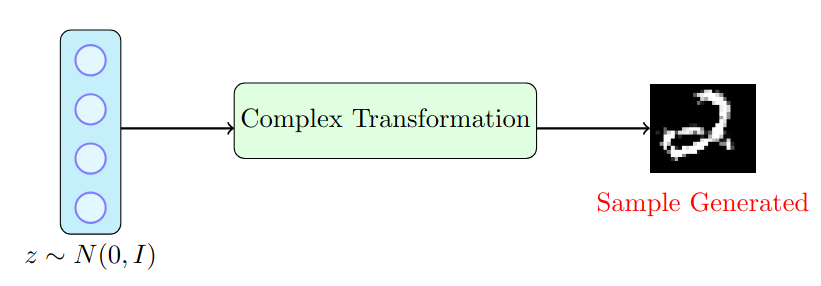
\includegraphics[width=0.8\textwidth]{../Images/gan1.png}
        \caption{Real vs Fake Images}
    \end{figure}

    We will sample $z \sim \mathcal{N}(0,\mathbb{I}_{d \times d})$ and pass it through a neural network (\textcolor{blue}{Generator}), and train it in such a way that output images looks similar to training images.
\end{frame}

\section*{Architecture}
\begin{frame}{Architecture}
    \begin{figure}
        \centering
        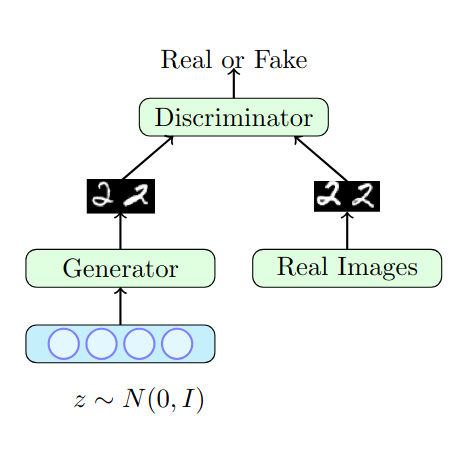
\includegraphics[width=0.45\textwidth]{../Images/gan2.png}
        \caption{GAN Architecture}
    \end{figure}
    To achieve what we just saw, another neural network is introduced, called the \textcolor{blue}{Discriminator}.
\end{frame}

\begin{frame}{Architecture}
    GAN's architecture consists of two neural networks:
    \begin{enumerate}
        \item \textcolor{blue}{Generator} $G(z;\phi)$
        \item \textcolor{blue}{Discriminator} $D(x;\theta)$
    \end{enumerate}

    where $\phi$ and $\theta$ are the parameters of the generator and discriminator respectively.
\end{frame}

\begin{frame}{Generator and Discriminator}
    The task of generator and discriminator is as follows:
    \begin{enumerate}
        \item Generator takes a random noise vector $z \sim \mathcal{N}(0,\mathbb{I}_{d \times d})$ and generates a image $X = G(z;\phi)$.

        \item Discriminator takes a image $X \sim p_{\text{data}}$ or $X = G(z;\phi)$ and outputs a probability $D(X;\theta)$ that $X$ is from the real data distribution.
    \end{enumerate}

    For convenience, we will denote $G(z;\phi)$ as $G_{\phi}(z)$ and $D(x;\theta)$ as $D_{\theta}(x)$.
\end{frame}

\begin{frame}{Types of GAN's}
    There are many types of GAN's:
    \begin{enumerate}
        \item \textcolor{blue}{DCGAN}: Deep Convolutional GAN
        \item \textcolor{blue}{WGAN}: Wasserstein GAN
        \item \textcolor{blue}{CGAN}: Conditional GAN
        \item \textcolor{blue}{Pix2Pix}: Image to Image Translation
        \item \textcolor{blue}{CycleGAN}: Cycle Consistent GAN
    \end{enumerate}
    We will be discussing the some of those in results section.
\end{frame}

\section*{Objective}
\begin{frame}{Generator Objective Function}
    We know that higher score from the discriminator means that the image is more likely to be from the real data distribution. \\

    \bigskip

    Hence for some $z \sim \mathcal{N}(0,\mathbb{I}_{d \times d})$, Generator objective can be written as:
    \begin{equation}
        \max_{\phi} \;\; log(D_{\theta}(G_{\phi}(z)))
    \end{equation}

    or we can also write it as:
    \begin{equation}
        \min_{\phi} \;\; log(1 - D_{\theta}(G_{\phi}(z)))
    \end{equation}
\end{frame}

\begin{frame}{Generator Objective Function}
    Hence we can write the generator objective function as:
    \begin{equation}
        \min_{\phi} \;\; \mathbb{E}_{z \sim \mathcal{N}(0,\mathbb{I}_{d \times d})} \left[ log(1 - D_{\theta}(G_{\phi}(z))) \right]
    \end{equation} 

    or equivalently:
    \begin{equation}
        \max_{\phi} \;\; \mathbb{E}_{z \sim \mathcal{N}(0,\mathbb{I}_{d \times d})} \left[ log(D_{\theta}(G_{\phi}(z))) \right]
    \end{equation}
\end{frame}

\begin{frame}{Discriminator Objective Function}
    Discriminator has to give high scores to images $\sim p_{\text{data}}$ and low scores to images $\sim G_{\phi}(z)$. Hence the objective function for discriminator can be written as: \\
    \begin{equation}
        \max_{\theta} \;\; \mathbb{E}_{x \sim p_{\text{data}}} \left[ log(D_{\theta}(x)) \right] + \mathbb{E}_{z \sim \mathcal{N}(0,\mathbb{I}_{d \times d})} \left[ log(1 - D_{\theta}(G_{\phi}(z))) \right]
    \end{equation}
\end{frame}

\begin{frame}{Overall Objective Function}
    The overall objective function for GAN can be written as:
    \begin{equation}
        \min_{\phi} \max_{\theta} \;\; \mathbb{E}_{x \sim p_{\text{data}}} \left[ log(D_{\theta}(x)) \right] + \mathbb{E}_{z \sim \mathcal{N}(0,\mathbb{I}_{d \times d})} \left[ log(1 - D_{\theta}(G_{\phi}(z))) \right]
    \end{equation}
    
    \begin{enumerate}
        \item Discriminator tries to maximize 2nd term where as Generator tries to minimize it (\textcolor{red}{Adversarial Training}).
        \item 1st term is independent of $\phi$ and hence can be ignored while training the generator.
    \end{enumerate}
\end{frame}

\section*{Training}
\begin{frame}{Training GAN's}
    Training GAN's is done by alternating between the following steps:
    \begin{enumerate}
        \item \textcolor{blue}{Train Discriminator}: Since we have to maximize w.r.t $\theta$, we use Gradient Ascent on:
        \begin{equation}
            \mathbb{E}_{x \sim p_{\text{data}}} \left[ log(D_{\theta}(x)) \right] + \mathbb{E}_{z \sim \mathcal{N}(0,\mathbb{I}_{d \times d})} \left[ log(1 - D_{\theta}(G_{\phi}(z))) \right]
        \end{equation}

        \item \textcolor{blue}{Train Generator}: Since we have to minimize w.r.t $\phi$, we use Gradient Descent on:
        \begin{equation}
            \mathbb{E}_{z \sim \mathcal{N}(0,\mathbb{I}_{d \times d})} \left[ log(1 - D_{\theta}(G_{\phi}(z))) \right]
        \end{equation}
    \end{enumerate}
\end{frame}

\begin{frame}{Algorithm for GAN Training}
    \begin{figure}
        \centering
        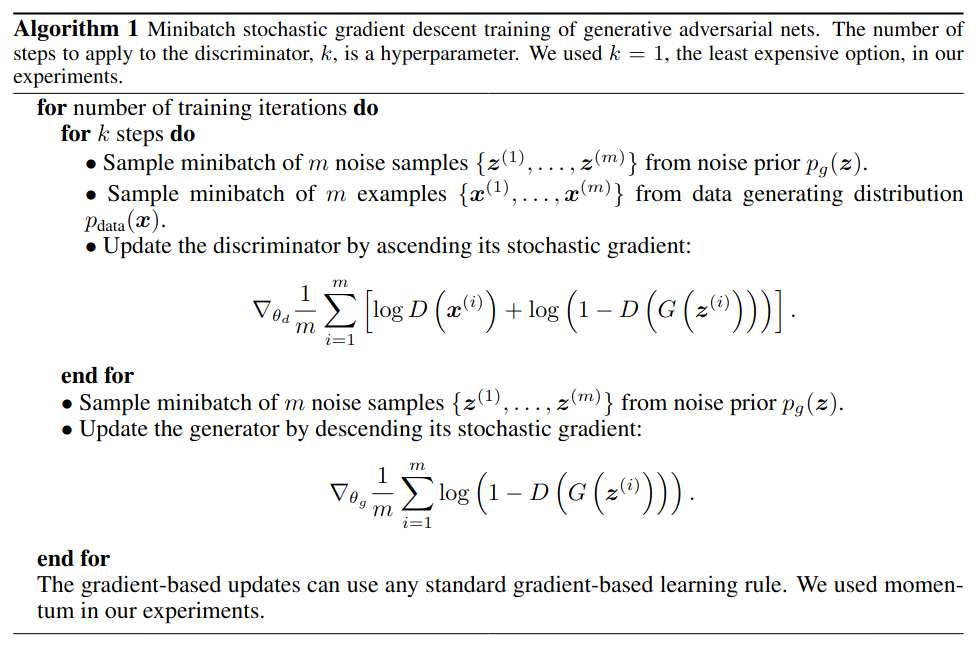
\includegraphics[width=1\textwidth]{../Images/gan4.png}
        \caption{GAN Training Algorithm}
    \end{figure}
\end{frame}

\begin{frame}{Generator Training}
    \begin{figure}
        \centering
        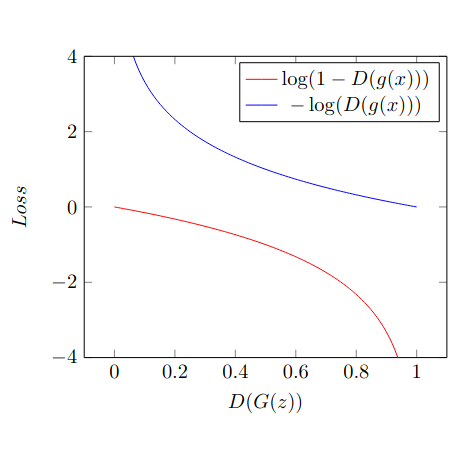
\includegraphics[width=0.4\textwidth]{../Images/gan3.png}
        \caption{Generator Training}
    \end{figure}
    In practice $log(1 - D_{\theta}(G_{\phi}(z)))$ may not provide enough gradient for the generator to learn because it will be close to 0 initially. 
\end{frame}

\begin{frame}{New Training Objective For Generator}
    We can use the following objective function for training the generator:
    \begin{equation}
        \max_{\phi} \;\; \mathbb{E}_{z \sim \mathcal{N}(0,\mathbb{I}_{d \times d})} \left[ log(D_{\theta}(G_{\phi}(z))) \right]
    \end{equation}
    
    Now in this case Gradients will flow better and the generator will learn faster.
\end{frame}

\section*{Results}
\begin{frame}{Generated Handwritten Digits}
    \begin{figure}
        \centering
        
\includegraphics[width=0.4\textwidth]{../Images/gan5.png}
        \caption{Generated Handwritten Digits}
    \end{figure}
    In this case both the generator and discriminator are feed forward neural networks.
\end{frame}

\begin{frame}{Generated Face Images}
    \begin{figure}
        \centering
        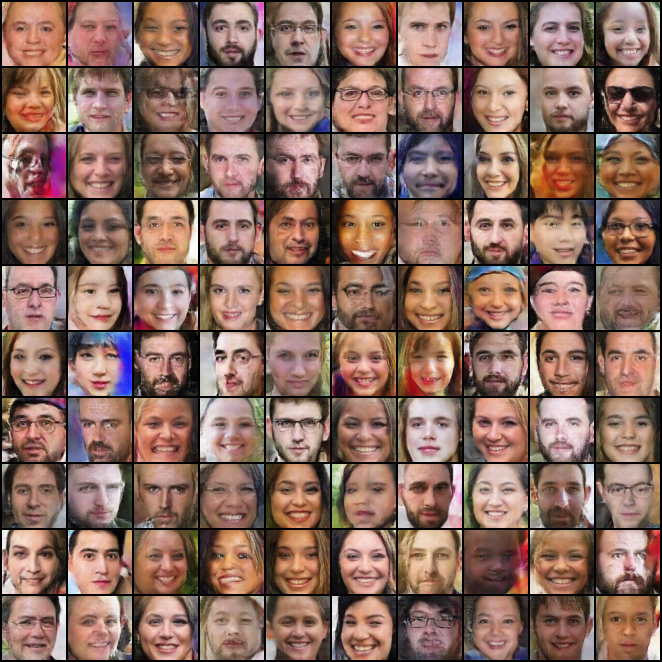
\includegraphics[width=0.4\textwidth]{../Images/gan6.png}
        \caption{Generated Face Images}
    \end{figure}
    In this case both the generator and discriminator are Convolutional Neural Networks.
\end{frame}

\begin{frame}{Generated Anime Characters}
    \begin{figure}
        \centering
        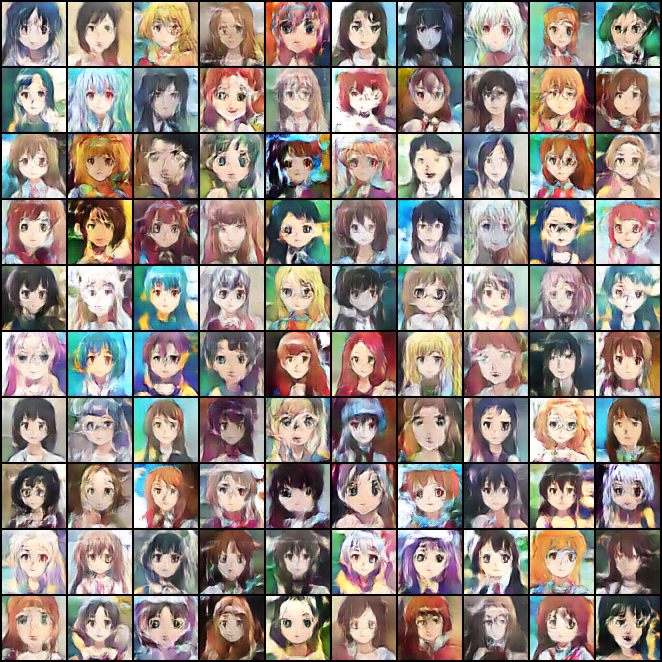
\includegraphics[width=0.4\textwidth]{../Images/gan7.png}
        \caption{Generated Anime Characters}
    \end{figure}
    In this case both the generator and discriminator are Convolutional Neural Networks
\end{frame}

\begin{frame}{Generated Animal Images}
    \begin{figure}
        \centering
        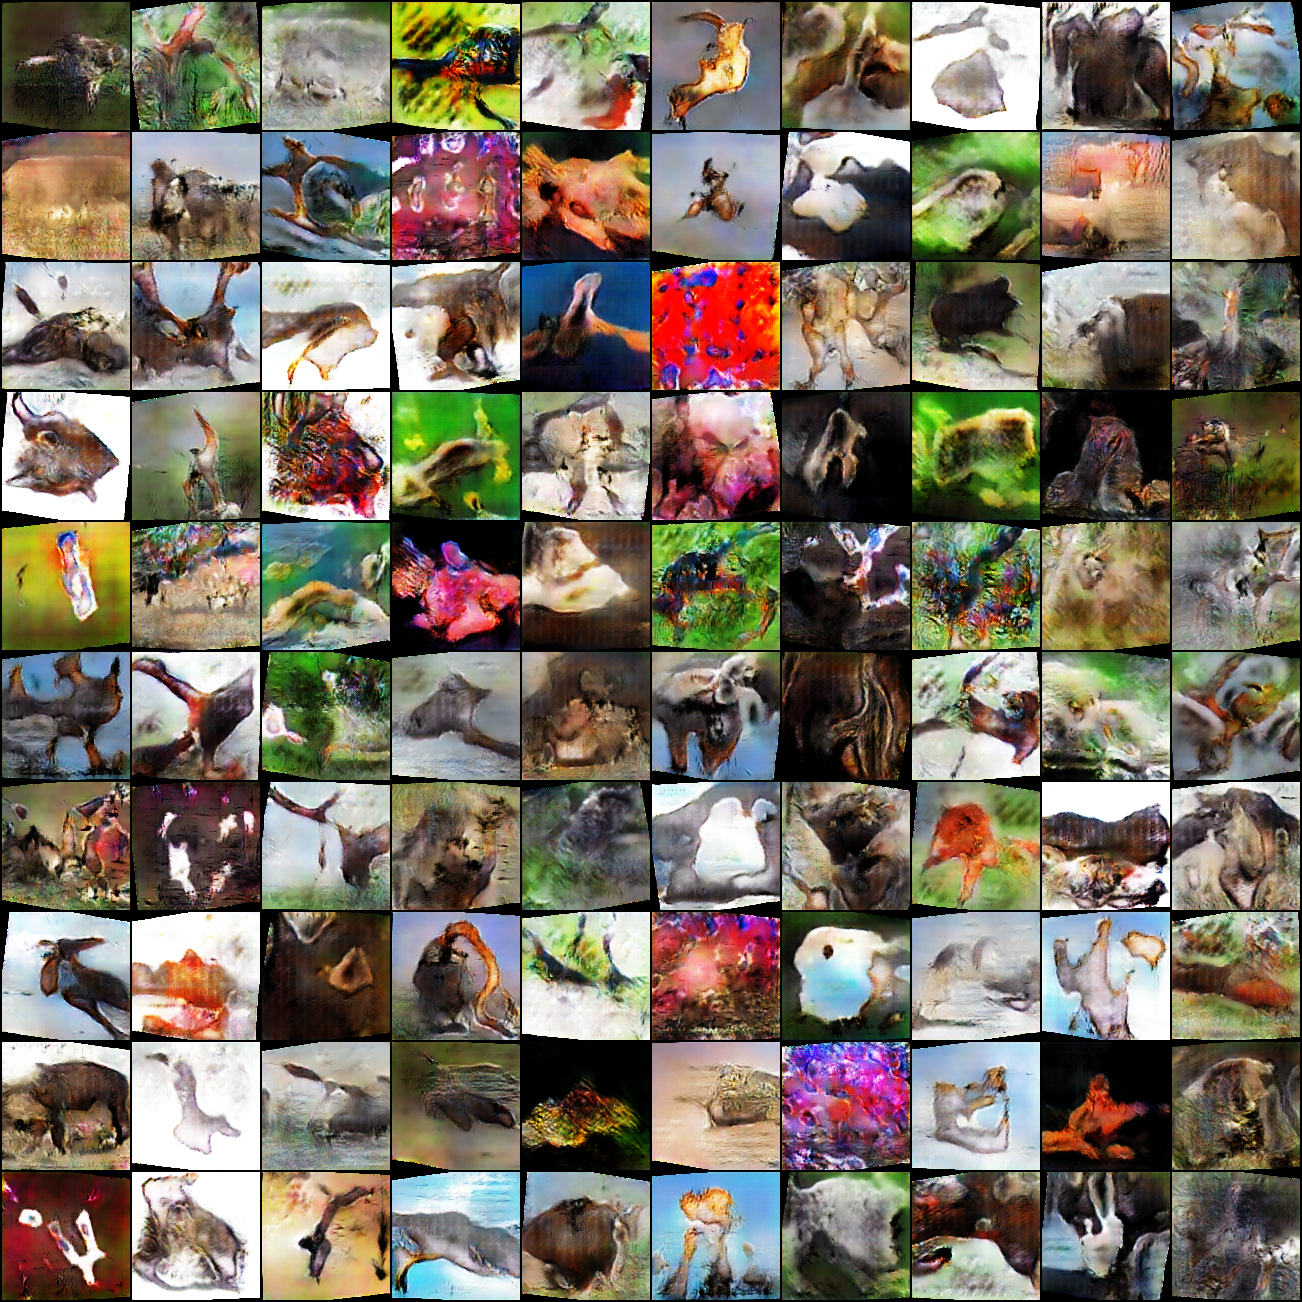
\includegraphics[width=0.4\textwidth]{../Images/gan8.png}
        \caption{Generated Animal Images}
    \end{figure}
    In this case both the generator and discriminator are Convolutional Neural Networks.
    
\end{frame}



%reference slide
\begin{frame}{References}
    \begin{thebibliography}{9}
        \bibitem{goodfellow2014}
        Ian Goodfellow, Jean Pouget-Abadie, Mehdi Mirza, Bing Xu, David Warde-Farley, Sherjil Ozair, Aaron Courville, Yoshua Bengio
        \textit{Generative Adversarial Networks}.
        arXiv:1406.2661, 2014.
        
        \bibitem{radford2015}
        Alec Radford, Luke Metz, Soumith Chintala
        \textit{Unsupervised Representation Learning with Deep Convolutional Generative Adversarial Networks}.
        arXiv:1511.06434, 2015.
        
        \bibitem{salimans2016}
        Tim Salimans, Ian Goodfellow, Wojciech Zaremba, Vicki Cheung, Alec Radford, Xi Chen
        \textit{Improved Techniques for Training GANs}.
        arXiv:1606.03498, 2016.
        
        \bibitem{arjovsky2017}
        Martin Arjovsky, Soumith Chintala, Léon Bottou
        \textit{Wasserstein
        GAN}.
        arXiv:1701.07875, 2017.
    \end{thebibliography}
\end{frame}

% thank you slide
\begin{frame}{Thank You!}
    \begin{center}
        \Huge Thank You!
    \end{center}
\end{frame}

\end{document}

